\documentclass[11pt,a4paper]{article}

% ---------- packages ----------
\usepackage[T1]{fontenc}
\usepackage[utf8]{inputenc}
\usepackage{lmodern}
\usepackage[margin=2.5cm]{geometry}
\usepackage{microtype}
\usepackage{amsmath,amssymb}
\usepackage{graphicx}
\usepackage{booktabs,tabularx,longtable,array,multirow}
\usepackage[table]{xcolor}
\usepackage{enumitem}
\usepackage{caption}
\usepackage{tikz}
\usetikzlibrary{positioning,arrows.meta}
\usepackage[numbers,sort&compress]{natbib}
\usepackage{xurl}
\usepackage[hidelinks]{hyperref}

\graphicspath{{figures/}{../literature/figures/}} % figures/ only needed on Overleaf
\setlist{nosep,leftmargin=*}
\setlength{\emergencystretch}{2em}
\captionsetup{font=small,labelfont=bf}
\renewcommand{\arraystretch}{1.15}

% ---------- project macros ----------
% Red placeholder: everything still to be filled in or checked.
\newcommand{\fillin}[1]{\textcolor{red}{[\textbf{TODO:} #1]}}
% Result that only exists after a run.
\newcommand{\pending}{\textcolor{red}{\textbf{[pending]}}}
% Record ID with its citation, e.g. \rec{C01} -> C01 [12].
\newcommand{\rec}[1]{#1~\citep{#1}}
\newcommand{\code}[1]{\texttt{\detokenize{#1}}}
\newcolumntype{L}[1]{>{\raggedright\arraybackslash}p{#1}}
\newcolumntype{Y}{>{\raggedright\arraybackslash}X}

\hypersetup{pdftitle={Does Topology Help? An Audit and Fair Re-evaluation of TDA Anomaly Detection for Systems and Security Telemetry}}

\begin{document}

% ---------- cover page ----------
\begin{titlepage}
  \centering
  \vspace*{1.5cm}
  {\Large \fillin{Institute name}\par}
  \vspace{0.3cm}
  {\large \fillin{Department}\par}
  \vspace{2cm}
  {\LARGE\bfseries Does Topology Help?\par}
  \vspace{0.4cm}
  {\Large An Audit and Fair Re-evaluation of Topological Data Analysis\\
  Anomaly Detection for Systems and Security Telemetry\par}
  \vspace{2cm}
  {\large Semester project report\par}
  \vspace{1.5cm}
  \begin{tabular}{rl}
    Submitted by: & Anirudh \fillin{full name} \\
    Roll number:  & \fillin{roll no.} \\
    Programme:    & \fillin{course and semester} \\
    Supervisor:   & \fillin{name, designation} \\
  \end{tabular}
  \vfill
  {\large \fillin{month} 2026\par}
\end{titlepage}

\begin{abstract}
\noindent
Topological data analysis (TDA) is increasingly proposed for anomaly detection on network, host and server telemetry. The usual argument is that topology captures ``shape'' that simple statistics miss. We test whether the published evidence supports that argument, and then test the argument ourselves.
First, we audit 95 records, of which 32 are core applications, against a 13-item rigour rubric. Only 4 of the 32 papers compare topology fairly, by swapping it for cheap features under the same data, split and detector: two lose, one ties and one shows a weak win. None tests against an adversary.
Second, we read the released code of six projects at pinned commits. Three of them use test information when choosing thresholds, detectors or training stops. One assigns random timestamps that then serve as the persistence filtration. A topology processor shipped in Fluent Bit does not count what its comment says it counts.
Third, we re-evaluate the claims under a preregistered protocol on SMD and CTU-13. On SMD, adding topological features to the same detector raises PR-AUC by 0.054 [0.035, 0.076], at about 1.6\,ms per window. \fillin{E1, E2, E4 and E5 results; the shape-versus-volume answer}.
\end{abstract}

\tableofcontents
\clearpage

\section{Problem and question}
\label{sec:intro}

\subsection{The claim}
Topological data analysis (TDA) describes the shape of data. Its main tool, persistent homology, records which connected pieces and loops appear in the data across scales and how long each one survives~\cite{edelsbrunner2002persistence,A01,carlsson2009topology}. Over the past decade, TDA has been applied to security and systems telemetry: darknet packets, network flows, host logs, malware call graphs and server metrics. These papers usually make the same argument. Attacks and faults change the \emph{structure} of the data: its rhythm, the coupling between signals, or the way hosts connect. Topology is meant to capture that structure where counts and averages cannot.

\subsection{The problem}
A detector that uses topological features can perform well for many reasons other than topology. The learner may be stronger. It may have been tuned more. The threshold may have been chosen with test labels. The benchmark itself may make detection easy. Only one experimental design isolates topology's contribution: keep the data, split, detector and tuning fixed, and \emph{replace} the topological features with cheap ones. We call this a \emph{swap test}.

Removing the topology branch from a model is not enough. Removal shows that the model needs \emph{some} extra input. It does not show that topology beats a cheap input of the same size. Comparing against other people's systems is weaker still, because the learner, the tuning and often the data split differ too.

\subsection{Research question}
\begin{quote}
\emph{Does topology add detection value over cheap features when evaluation is fair, and if it does, for which kinds of anomaly?}
\end{quote}
We split this question into three predictions, fixed before any data was opened (Section~\ref{sec:prereg}):
\begin{description}
  \item[P1] Topology adds value on \emph{shape} anomalies: changes in rhythm, coupling or connectivity.
  \item[P2] Topology adds \emph{no} value on \emph{volume} anomalies (changes in rate or magnitude) or \emph{identity} anomalies (a specific host or port).
  \item[P3] Published TDA results shrink under fair evaluation.
\end{description}

\subsection{Contributions}
\begin{enumerate}
  \item \textbf{Literature audit.} We screened 95 records and scored the 32 core applications on a 13-item rubric (R1--R13). Only 4 of the 32 swap-test topology: 2 lose, 1 ties and 1 shows a weak win. No paper tests against an adversary who knows the method (Section~\ref{sec:audit}).
  \item \textbf{Code audit.} We read the released code of six projects at pinned commits. Three releases use test information when setting thresholds, choosing detectors or stopping training. One uses random timestamps as its filtration. Fluent Bit's \code{tda} processor counts something other than what its comment states (Section~\ref{sec:code}).
  \item \textbf{Fair re-evaluation.} We re-test the claims under a preregistered protocol, using released code and public data: SMD for systems and CTU-13 for security (Section~\ref{sec:exp}).
  \item \textbf{Mechanism test.} We inject controlled shape and volume anomalies into SMD to test \emph{why} topology helps or fails (Sections~\ref{sec:exp} and~\ref{sec:why}).
\end{enumerate}

\paragraph{What this report does not claim.} We do not propose a new detector. We do not claim that topology is useless. The claim under test is narrower: that topological features add detection value \emph{beyond cheap features}, under evaluation rules that avoid test leakage.

\paragraph{Organisation.} Section~\ref{sec:background} explains what TDA can and cannot capture. Section~\ref{sec:method} describes the audit method and the preregistered protocol. Sections~\ref{sec:audit} and~\ref{sec:code} report the literature and code audits. Section~\ref{sec:exp} reports experiments E1--E5. Section~\ref{sec:why} interprets them through the shape-versus-volume lens, and Section~\ref{sec:limits} lists limitations.

\section{Background: what TDA can and cannot capture}
\label{sec:background}

This section gives just enough TDA to follow the rest of the report. It ends with the argument behind P1 and P2: which kinds of change a topological summary can see at all, and which of them cheap statistics already see.

\subsection{Persistent homology}
Start with a finite set of points $X$, for example the samples in one telemetry window. For a scale $\varepsilon \ge 0$, the \emph{Vietoris--Rips complex} $\mathrm{VR}_\varepsilon(X)$ contains a simplex (edge, triangle and so on) for every group of points that are pairwise within distance $\varepsilon$. As $\varepsilon$ grows, the complexes only gain simplices, so they form a nested sequence called a \emph{filtration}.

Along the filtration, topological features appear and disappear:
\begin{itemize}
  \item an \textbf{$H_0$ class} is a connected component. Every point starts as its own component, and components merge as $\varepsilon$ grows;
  \item an \textbf{$H_1$ class} is a loop: a cycle of edges that is not yet filled in by triangles.
\end{itemize}
Each class has a birth scale $b$ and a death scale $d$. The multiset of pairs $(b,d)$ is the \emph{persistence diagram}; drawn as intervals, it is the \emph{barcode}~\cite{edelsbrunner2002persistence,A01}. Long bars are read as real structure and short bars as noise.

Two properties matter for detection:
\begin{itemize}
  \item \textbf{Stability.} Small changes to the input move the diagram only a little, as measured by the bottleneck distance~\cite{A02}. This makes diagrams robust to noise. It also means that a small anomaly produces only a small change in the diagram.
  \item \textbf{Invariance.} Rips persistence depends only on the pairwise distances between points. Translating the whole cloud, or relabelling its points, leaves the diagram unchanged. Scaling every distance by a factor $c$ scales every birth and death by $c$.
\end{itemize}

Detectors need fixed-length vectors, so diagrams are summarised: bar counts and lifetime statistics, persistent entropy, Betti curves (the number of alive classes at each scale), persistence landscapes~\cite{A03} or persistence images~\cite{A04}. We compute Rips persistence with Ripser~\cite{A06}.

\subsection{From time series to point clouds}
A telemetry window is a sequence, not a point cloud. The standard bridge is \emph{delay embedding}. A window $x_1,\dots,x_w$ becomes the points
\[
  v_i = \bigl(x_i,\; x_{i+\tau},\; \dots,\; x_{i+(m-1)\tau}\bigr), \qquad i = 1,\dots,w-(m-1)\tau ,
\]
with embedding dimension $m$ and delay $\tau$~\cite{takens1981}. A periodic signal traces a closed curve in this space, so it leaves a long $H_1$ bar. The size and roundness of that loop depend on the amplitude, the period, the window length and $\tau$~\cite{A05}. TAME~\cite{D02} and Fluent Bit's \code{tda} processor~\cite{fluentbit_pr11250} both use $m=3$, $\tau=1$, and so do we (Section~\ref{sec:prereg}). With $w=60$, each window gives 58 points.
Our F3 embeds all 38 SMD channels \emph{jointly}: each 60-step window becomes one cloud of 58 points in 114 dimensions, with one $H_0$ and one $H_1$ diagram per window.

Other constructions appear in the literature:
\begin{itemize}
  \item TADA~\cite{H04} builds its filtration from the dependence structure \emph{between channels} within a window, rather than from a delay embedding. \fillin{confirm against the \code{tdaad} source at the pinned commit}
  \item \textbf{Mapper}~\cite{A07} covers the range of a ``lens'' function with overlapping intervals, clusters the points in each interval and links clusters that share points. The result is a graph for visual exploration, not a detector.
  \item \textbf{Zigzag persistence}~\cite{I01} tracks classes through a \emph{sequence} of spaces that can both grow and shrink, such as the hypergraph of who talks to whom in consecutive windows. I03~\citep{I03} uses it on network flows.
\end{itemize}

\subsection{What a topological summary can see}
\label{sec:cansee}
Table~\ref{tab:see} applies the invariance argument to the anomaly types we inject in E5 (Section~\ref{sec:prereg}). It reasons about a Rips summary of one window, with every point inside the window. Two conclusions follow.
\begin{itemize}
  \item \textbf{Volume and identity.} Changes of level, size or identity are either invisible to topology or visible to much cheaper statistics. This is the basis of P2.
  \item \textbf{Shape.} Changes of rhythm and coupling \emph{are} visible to topology. Because F3 embeds the channels jointly, this includes S2 and S3. But simple structure features, such as autocorrelation, spectral peaks and correlation matrices, see them too. P1 therefore asks whether topology adds value \emph{beyond those features}, and that is why our baseline F2 includes them.
\end{itemize}

\begin{table}[ht]
\centering\small
\caption{What a Vietoris--Rips summary of a delay-embedded window can see, by anomaly type. ``Cheap feature'' names a non-topological statistic in our F1/F2 sets that responds to the same change. This is a reasoning aid, not a result.}
\label{tab:see}
\begin{tabularx}{\linewidth}{@{}L{2.3cm}L{2.6cm}YL{2.8cm}@{}}
\toprule
Type & Change & Effect on the diagram & Cheap feature that also responds \\
\midrule
Volume (V1) & Level shift over the whole window & None: the cloud is translated, and translation leaves the diagram unchanged & Mean \\
Volume (V1) & Level shift starting mid-window & The cloud splits into two groups, giving one long $H_0$ bar & Mean, variance \\
Volume (V2) & A few large spikes & Outlying points give long-lived $H_0$ bars & Maximum, variance \\
Volume (V3) & Spread scaled by $c$ around the mean & Every birth and death scales by $c$; nothing changes if summaries are scale-normalised & Variance \\
Shape (S1) & Period changed & The loop in the embedding changes size and shape & Spectral peak, autocorrelation \\
Shape (S2) & One coupled channel phase-shifted & Visible only if the channels are embedded \emph{jointly}; a per-channel embedding of a shifted sine is unchanged & Lagged cross-correlation, correlation summary \\
Shape (S3) & Coupling broken; marginal kept & Joint cloud loses its structure; a per-channel cloud changes little & Correlation summary \\
Identity & Activity tied to a specific host or port & None: relabelling vertices leaves topology unchanged & Per-destination counts \\
\bottomrule
\end{tabularx}
\end{table}

\paragraph{Cost.} The number of Rips simplices grows quickly with the number of points and the maximum dimension. With 58 points and homology up to $H_1$, one window takes well under a second in Ripser; measured costs are in Section~\ref{sec:exp}. The cost matters more for streaming claims (rubric item R7, Section~\ref{sec:rubric}), where many windows per second are needed.

\section{Method}
\label{sec:method}

The project has two halves (Figure~\ref{fig:pipeline}). The audit asks what the published evidence shows. The re-evaluation tests the claims ourselves under rules that were fixed before any data was opened.

\begin{figure}[ht]
\centering
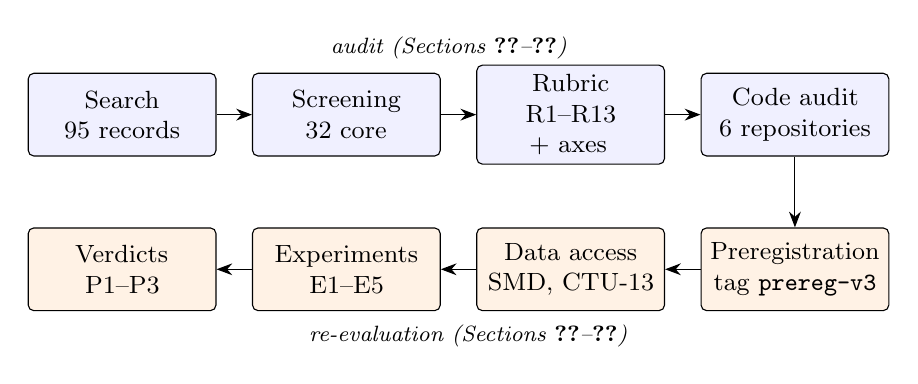
\begin{tikzpicture}[
  box/.style={draw, rounded corners=2pt, align=center, font=\small, minimum height=1.05cm, text width=2.15cm, fill=#1},
  box/.default=white, >={Stealth[length=2mm]}, node distance=0.45cm]
  \node[box=blue!6] (s) {Search\\95 records};
  \node[box=blue!6, right=of s] (c) {Screening\\32 core};
  \node[box=blue!6, right=of c] (r) {Rubric\\R1--R13 + axes};
  \node[box=blue!6, right=of r] (k) {Code audit\\6 repositories};
  \node[box=orange!10, below=0.9cm of k] (p) {Preregistration\\tag \code{prereg-v3}};
  \node[box=orange!10, left=of p] (d) {Data access\\SMD, CTU-13};
  \node[box=orange!10, left=of d] (e) {Experiments\\E1--E5};
  \node[box=orange!10, left=of e] (v) {Verdicts\\P1--P3};
  \draw[->] (s) -- (c); \draw[->] (c) -- (r); \draw[->] (r) -- (k);
  \draw[->] (k) -- (p); \draw[->] (p) -- (d); \draw[->] (d) -- (e); \draw[->] (e) -- (v);
  \node[font=\footnotesize\itshape, above=0.05cm of c, xshift=1.3cm] {audit (Sections~\ref{sec:audit}--\ref{sec:code})};
  \node[font=\footnotesize\itshape, below=0.05cm of d, xshift=-1.3cm] {re-evaluation (Sections~\ref{sec:exp}--\ref{sec:why})};
\end{tikzpicture}
\caption{Project pipeline. The audit (top) motivates the preregistered re-evaluation (bottom). No data was opened before the preregistration was committed and tagged.}
\label{fig:pipeline}
\end{figure}

\subsection{Search}
\label{sec:search}
The search ran in three rounds:
\begin{enumerate}
  \item \textbf{Initial audit} (search cut-off 14 October 2026): 76 records.
  \item \textbf{Round 2} (13--15 November): 119 distinct logged queries, namely 69 web searches, 23 OpenAlex, 11 Semantic Scholar API, 10 publisher sites, 5 arXiv and 1 DBLP. It included separate sweeps for network security, host security and systems telemetry, plus a Chinese-language and boundary pass.
  \item \textbf{Round 3} (15--16 November): forward citations from seven seed papers, plus targeted gap searches.
\end{enumerate}
The final set has 95 records. Semantic Scholar refused or rate-limited some requests, so citation expansion in round 2 was incomplete. The search for earlier critical reviews was also not completed. The closest existing reviews are Davies~\cite{P01}, a catalogue of TDA in cybersecurity, and Georgiou et al.~\cite{georgiou2026tda}, a broad TDA survey that gives security one short section. Neither audits evaluation practice. Our claim that no critical review exists therefore has medium-low confidence.

\paragraph{Use of AI assistants.} Searches and first-pass extraction were done with AI research assistants (Claude) working from fixed written protocols. Each number in the records names its source table or section. Each claim is marked as \emph{Author} (what the paper says) or \emph{Assessment} (our judgement). The author's own check is the blind re-scoring in Section~\ref{sec:recheck}. \fillin{confirm wording; full AI-use note in an appendix}

\subsection{Screening and scope}
\label{sec:scope}
\begin{itemize}
  \item \textbf{Core security clusters.} S1 network flows and packets, S2 darknet traffic, S3 host logs, S4 activity and provenance graphs, S5 malware, S6 encrypted-traffic and IoT fingerprinting, S7 wireless networks, S8 DNS.
  \item \textbf{Core systems clusters.} I1 server and cloud metrics, I2 big-data jobs, I3 HPC, I4 traces and serverless, I5 OS and hardware, I6 network operations.
  \item \textbf{Boundary clusters.} These are kept out of the core counts: B1 cyber-physical systems and the grid, B2 ledgers, B3 software artefacts, B4 poisoning and federated learning, and social-media bots.
\end{itemize}

A record is \textbf{included as core} only if it meets both conditions:
\begin{enumerate}
  \item it computes a genuine topological invariant or construction: persistent homology and its summaries, Mapper or Reeb graphs, zigzag or multiparameter persistence, directed constructions, sheaf or Hodge methods, or homological deep learning;
  \item it applies that invariant to in-scope data.
\end{enumerate}

Three terminology traps were screened out: ``topology'' meaning a service map or attack graph, ``persistence'' in the temporal sense, and ordinary graph metrics labelled as topological.

Table~\ref{tab:screening} gives the outcome. Of the 32 core papers, 24 were read in full and 8 only as abstracts, because the full text was closed or unavailable.

\begin{table}[ht]
\centering\small
\caption{Screening outcome for the 95 records.}
\label{tab:screening}
\begin{tabular}{@{}lr@{}}
\toprule
Status & Records \\
\midrule
Core application (S1--S8, I1--I6) & 32 \\
Boundary application (B1--B4, social bots) & 14 \\
Not an application (theory, method, review or benchmark context) & 43 \\
Core method on modelled data only (E02) & 1 \\
Candidate, inclusion unverified (B10) & 1 \\
Merged into a later version (D05 into D02) & 1 \\
Excluded: no homology computed (J06); Mapper described but never shown on data (D03) & 2 \\
Out of scope (M01, wind turbines) & 1 \\
\midrule
Total & 95 \\
\bottomrule
\end{tabular}
\end{table}

\subsection{Rubric and coding axes}
\label{sec:rubric}
Each core paper was scored on the 13 items in Table~\ref{tab:rubric}, each as Y (yes), P (partial), N (no), U (unknown: not reported, or text not readable) or NA (not applicable). The items follow established pitfalls in machine learning for security~\cite{sommer2010closed,arp2022dos} and in time-series anomaly benchmarks~\cite{Q04,kim2022rigorous}.

\begin{table}[ht]
\centering\small
\caption{Rigour rubric applied to each core paper.}
\label{tab:rubric}
\begin{tabularx}{\linewidth}{@{}lY@{}}
\toprule
Item & Criterion \\
\midrule
R1 & Matched non-topological baseline: same data, split, learner and tuning \\
R2 & Replacement ablation: topology \emph{swapped} for cheap features, not merely removed \\
R3 & Leakage-safe split: separated by time or entity; preprocessing and thresholds fitted on training data only \\
R4 & Threshold chosen without test labels or test prevalence \\
R5 & Prevalence-aware metrics: PR-AUC, precision at fixed recall, or false alarms per unit time \\
R6 & Uncertainty measured across independent units (hosts, days, scenarios), not only across seeds \\
R7 & Cost reported; for ``real-time'' claims, latency at a stated event rate \\
R8 & Robustness tests: noise, drift or missing data \\
R9 & An adversary who knows the method \\
R10 & Known benchmark flaws acknowledged, or corrected data used \\
R11 & Interpretation claims supported by evidence \\
R12 & Code released \\
R13 & Data available \\
\bottomrule
\end{tabularx}
\end{table}

Each core paper was also coded on four axes:
\begin{itemize}
  \item \textbf{OUT}: Helped, Tied, Lost, Mixed or Untested, against the \emph{best non-topological comparator in the same paper}. ``Tied'' means within the reported noise, or less than one point apart with no statistical test.
  \item \textbf{USE}: Detection, Exploration (visual analytics or triage), Efficiency (sampling, data reduction or augmentation), or Component (persistent homology inside a larger learned model).
  \item \textbf{CHG}: what the target anomaly mainly changes: Shape, Volume, Identity, Content, Mixed or Unclear.
  \item \textbf{ISO}: how the paper isolates topology's contribution: Replacement (a swap test), Removal-only, or Not-isolated.
\end{itemize}
For reporting, papers are grouped by how close they came to a swap test: \textbf{A} swapped; \textbf{B} topology only removed; \textbf{C} compared only with other people's systems; \textbf{D} no comparison; \textbf{E} known only from the abstract or from code.

\subsection{Self re-check}
\label{sec:recheck}
To estimate coding reliability, the author re-scored 7 core papers blind on R1--R13 and OUT/ISO, without looking at the existing scores. Agreement was \fillin{xx\%} of items (\fillin{n of N}). Disagreements were \fillin{resolved how; what changed}.

\subsection{Code audit}
\label{sec:codemethod}
For papers with released code, we read the repository at a fixed commit and recorded the file and line numbers behind every claim. Every statement in Section~\ref{sec:code} describes what the \emph{released code} does, not what the authors ran for their paper. We do not call any result invalid. We state what the code does and what follows from it.

\subsection{Preregistered re-evaluation}
\label{sec:prereg}
The experiment plan was written down and committed \emph{alone} to a public repository, tagged \code{prereg-v3}, before any SMD or CTU-13 data was opened~\cite{nosek2018prereg}. \fillin{commit hash 773d00d and tag date; confirm the tag is on the remote} Version 3 replaced version 2 (16 November) on 19 November, still before data access. The change log is kept in the preregistration. Any change after data access goes into a deviations log with its date, reason and affected results, and both the original and the amended results are reported.

\paragraph{Datasets.}
\begin{itemize}
  \item \textbf{SMD}~\cite{su2019smd}: 28 server machines, 38 metrics each, with the official train and test files.
    \begin{itemize}
      \item Training data is treated as normal.
      \item Validation is the last 20\% of each machine's training data.
      \item Windows are 60 samples long, with a step of 10.
      \item A window is \emph{positive} if a labelled point falls in its final 10 samples, and \emph{normal} if it contains no labelled point; any other window is dropped.
    \end{itemize}
  \item \textbf{CTU-13}~\cite{garcia2014ctu}: labelled bidirectional NetFlow from botnet captures.
    \begin{itemize}
      \item Windows are \emph{per host}: 10-second bins, 60 bins per window, a step of 30 bins.
      \item A window is \emph{positive} if it belongs to an infected host and contains a botnet flow, and \emph{normal} if it belongs to a labelled normal host, contains a normal flow and contains no botnet flow.
      \item Splits are leave-one-scenario-out.
    \end{itemize}
\end{itemize}

\paragraph{Feature sets.} All sets are computed on the same windows, with every scaler and every PCA fitted on training data only.
\begin{itemize}
  \item \textbf{F1 Simple}: per-channel sum, mean, variance and number of unique values. CTU-13 adds flow, byte, packet, destination-IP and destination-port counts.
  \item \textbf{F2 Simple-structure}:
    \begin{itemize}
      \item correlation summaries;
      \item periodicity: FFT peak share and maximum autocorrelation;
      \item PCA reconstruction error.
    \end{itemize}
    CTU-13 adds destination-graph components, cycle rank and degree statistics.
  \item \textbf{F3 Topology}: delay embedding ($m=3$, $\tau=1$) of all channels jointly (58 points in 114 dimensions per SMD window), Rips persistence in $H_0$ and $H_1$, and 32 fixed summaries (bar counts, lifetime statistics, persistent entropy, and Betti curves at 10 multiples of the median pairwise distance). Nothing is tuned.
  \item \textbf{F5 Fluent Bit-style}: replicates the \code{tda} processor to output $\beta_0,\beta_1,\beta_2$ (exploratory; Section~\ref{sec:fluentbit}).
  \item \textbf{Z and Z-control} (CTU-13): zigzag persistence over per-host hypergraphs, against I03's own control of edges, vertices, components and diameter.
\end{itemize}

\paragraph{Detector, threshold and metrics.}
\begin{itemize}
  \item \textbf{Detector.} Every feature set uses the same Isolation Forest~\cite{liu2008iforest} with fixed defaults: 300 trees and automatic sample size. It is trained on normal windows and run with 5 seeds. Nothing is tuned, because SMD validation data contains no anomalies, so PR-AUC cannot be used to select settings.
  \item \textbf{Threshold.} The alarm threshold is set at a 1\% false-alarm rate on validation windows. Test labels are never used, and there is no point adjustment~\cite{kim2022rigorous}.
  \item \textbf{Metrics.} The primary metric is PR-AUC. We also report recall at the threshold, false alarms per day (consecutive alarm windows count as one event), ROC-AUC (for comparison with published numbers) and runtime per window.
\end{itemize}

\paragraph{Experiments.} Table~\ref{tab:exps} lists the experiments.

\begin{table}[ht]
\centering\small
\caption{Preregistered experiments.}
\label{tab:exps}
\begin{tabularx}{\linewidth}{@{}lY@{}}
\toprule
ID & Description \\
\midrule
E1 & TAME~\cite{D02} as released, unchanged, compared with its reported SMD ROC-AUC of 0.808. Timebox: 2 days. \\
E2 & Fair re-test on SMD of TADA~\cite{H04,tdaad_repo}, PHANTOM~\cite{phantom_repo} and TAME. TAME is fixed in two ways: our threshold rule replaces its test-prevalence threshold, and its Isolation Forest variant is chosen \emph{in advance}. These run alongside our F1+F2 and F1+F2+F3 pipelines. \\
E3 & Swap test on SMD with the same detector: F1, F1+F2, F1+F3, F1+F2+F3 and F5. \\
E4 & CTU-13: F1+F2 against F1+F2+F3, and Z against Z-control. Zigzag timebox: 3 days, with a preregistered fallback. \\
E5 & Controlled injections into normal SMD test segments, three shape types (S1 period change, S2 phase shift, S3 correlation break) and three volume types (V1 level shift, V2 spikes, V3 variance scaling), each at three magnitudes. Each type compares F1+F2 against F1+F2+F3. \\
\bottomrule
\end{tabularx}
\end{table}

\paragraph{Decision rules.} The main gain is
\[
  \Delta = \text{PR-AUC}(\text{F1+F2+F3}) - \text{PR-AUC}(\text{F1+F2}),
\]
and the swap gain is
\[
  \Delta_s = \text{PR-AUC}(\text{F1+F3}) - \text{PR-AUC}(\text{F1+F2}).
\]
Confidence intervals come from a 95\% cluster bootstrap (2{,}000 resamples), clustered over machines (SMD) or scenarios (CTU-13), after averaging across seeds. A cell is judged:
\begin{itemize}
  \item \textbf{Helps} if $\Delta>0$ and the interval excludes 0;
  \item \textbf{No added value} if the whole interval lies inside $\pm 0.02$;
  \item \textbf{Inconclusive} otherwise, including any cell with fewer than 20 positive or 20 normal test windows.
\end{itemize}
The predictions are judged as follows:
\begin{itemize}
  \item \textbf{P1} is supported if $\Delta$ ``helps'' for at least 2 of the 3 shape types at the decision magnitude, and refuted if at least 2 show ``no added value''.
  \item \textbf{P2} is supported if all three volume types show ``no added value''. It is refuted if any volume type ``helps'' with $\Delta \ge 0.02$ after Bonferroni correction.
  \item \textbf{P3} compares TAME under E2 with E1.
\end{itemize}
F5, TADA and PHANTOM are reported descriptively and enter no verdict.

\paragraph{Deviations so far.}
\begin{itemize}
  \item CTU-13 scenario 10 (capture 51) ships without a \code{.binetflow} file, so it is excluded and 12 scenarios remain.
  \item F5 follows the literal \code{tda.c} code, including its differencing of gauges (Section~\ref{sec:fluentbit}). This was logged before any results were seen.
\end{itemize}
The full log is in Appendix~\ref{app:deviations}.

\section{Audit results}
\label{sec:audit}

\subsection{The evidence base}
The 32 core papers span 2010--2026, and 21 of them appeared in 2022 or later. 22 are peer-reviewed, 9 are preprints and 1 is grey literature.

\begin{itemize}
  \item \textbf{Security dominates.} 24 papers are on security telemetry. Network flows (S1) are the largest cluster, with 10 papers.
  \item \textbf{Systems telemetry is thin.} Only 8 papers are on systems telemetry, and 4 of those (I1) evaluate on generic multivariate benchmarks such as SMD rather than on an operational system.
  \item \textbf{Use.} Topology is used for detection in 14 papers, for visual exploration in 8, as a component inside a larger learned model in 8, for efficiency in 1, and the use is unclear in 1.
\end{itemize}

\subsection{Outcomes: how often does topology win, and against what?}
Figure~\ref{fig:evidence} and Table~\ref{tab:outcomes} summarise the outcomes. Across all 32 papers, topology helped in 5, tied in 4, gave mixed results in 2 and lost in 3. In 12 papers it was never compared with anything. For the remaining 6, the outcome is known only from an abstract or from released code (3), or could not be determined (3).

The headline counts hide the main problem: \emph{what} topology was compared against. Panel~(b) of Figure~\ref{fig:evidence} splits the 14 full-text papers that make any comparison by how they isolate topology. Only the four replacement studies (group A) can show that topology itself adds value. Of those, two lost, one tied and one gave a weak win.

\begin{figure}[ht]
\centering
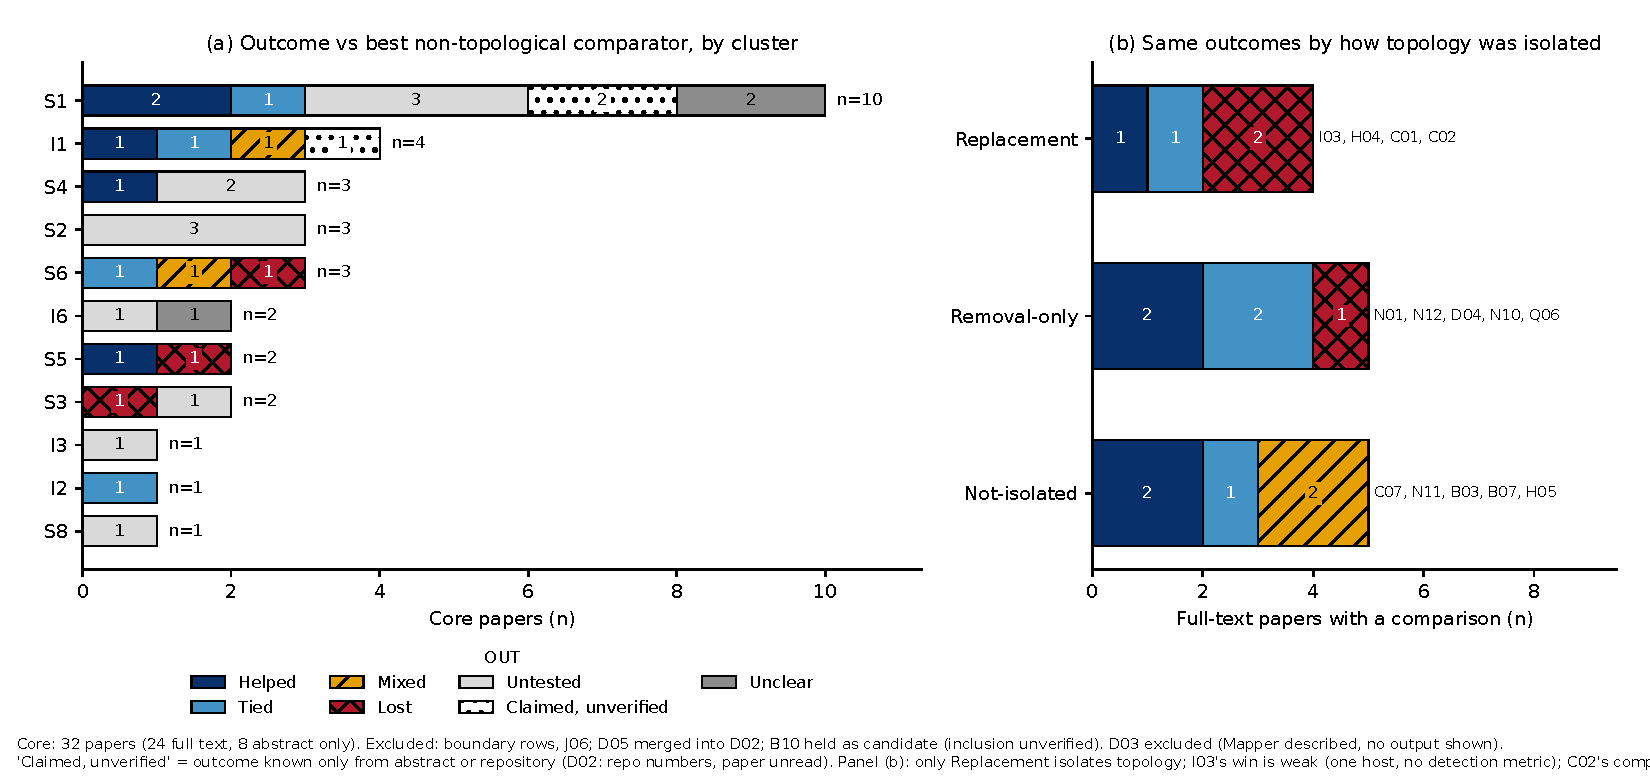
\includegraphics[width=\linewidth]{fig1_evidence_map.pdf}
\caption{Evidence map of the 32 core papers. (a) Outcome against the best non-topological comparator in the same paper, by cluster. (b) Outcomes of the 14 full-text papers that make a comparison, split by how they isolate topology. Only \emph{Replacement} is a swap test.}
\label{fig:evidence}
\end{figure}

\begin{table}[ht]
\centering\small
\caption{The 32 core papers grouped by study design (paper-by-paper dossier).}
\label{tab:outcomes}
\begin{tabularx}{\linewidth}{@{}lL{3.5cm}rYL{3.2cm}@{}}
\toprule
Group & Design & $n$ & Papers & Outcome \\
\midrule
A & Topology swapped for cheap features & 4 & C01, C02, H04, I03 & 2 lost, 1 tied, 1 weak win \\
B & Topology only removed & 5 & N01, N12, D04, N10, Q06 & 2 helped, 2 tied, 1 lost \\
C & Compared with other people's systems & 5 & C07, N11, B03, B07, H05 & 2 helped, 1 tied, 2 mixed \\
D & No comparison & 10 & B01, B08, D01, I02, J07, G01, I04, J05, C06, Q05 & untested \\
E & Abstract or code only & 8 & D02, N03, C08; N07, N09, B09; B05, B06 & 3 claimed, 3 unclear, 2 untested \\
\bottomrule
\end{tabularx}
\end{table}

\paragraph{Group A: the four swap tests.}
\begin{itemize}
  \item \textbf{\rec{C01}, host logs.} Persistent-homology features were compared with count features, using the same random forest and 10-fold cross-validation, on two synthetic log datasets and two graph constructions. Topology scored below the best non-topological feature set in all four settings, by 3.6 to 9.1 F1 points. For example, it reached 66.56 against 72.53 for counts.
    \emph{Caveat:} the data is synthetic and balanced, and the random folds likely overlap between training and test.
    This is the cleanest test in the literature, and topology lost.
  \item \textbf{\rec{C02}, malware.} Persistence-diagram features were swapped for PCA, UMAP and t-SNE features under the same tree learners, on CIC-MalMem-2022. The diagram features reached a detection rate of ``over 80\% on average''; UMAP and t-SNE reached 99--100\%. Extracting diagram features took 24.7\,s, against 1.08\,s for PCA.
    \emph{Caveat:} the diagram arm appears to be trained on homology-group labels rather than malware labels, so the comparison is not like-for-like.
    We code this as a loss of doubtful validity.
  \item \textbf{\rec{H04}, TADA on Exathlon (big-data jobs).} TADA ranked first on 5 of the 15 tabulated problems (by Range PR-AUC). The paper's own statistical ranking places it third, behind a non-topological method and Atol-IF, a related topological pipeline. We code this as a tie.
  \item \textbf{\rec{I03}, zigzag persistence on DARPA OpTC flows.} An autoencoder on zigzag features was compared with the same autoencoder on the authors' own summary statistics (edges, vertices, components, diameter). For one host, the malicious-to-benign reconstruction-loss ratio was about 36 with zigzag features and about 7.5 with summary statistics, and the zigzag spike matched the first attack in time.
    \emph{Caveats:} only one host is tabulated, with one seed, on one day. There is no threshold and no detection metric. The second attack group was missed. OpTC's benign activity is simulated.
    This is the only swap-test win, and it is weak. E4 re-tests the idea on CTU-13.
\end{itemize}

\paragraph{Group B: removal only.} These papers delete the topology branch and show that the full model scores higher:
\begin{itemize}
  \item \rec{N01}: F1 0.994 against 0.930 without persistent homology, in a single run;
  \item \rec{N12}: +0.5 to +2.2 F1 points;
  \item \rec{D04}: +3.8 average F1 points over the version without topology.
\end{itemize}
This shows that the model benefits from the extra input. It does not show that topology beats a cheap input of the same size. Against external baselines, the same papers are close. TopoGDN (D04) beats TranAD by 0.54 F1 points on SMD and 0.85 on MSL, in single runs without variance. Its removal ablation also disagrees with its own main table on SWaT. In \rec{N10}, the hybrid model, an LSTM alone and an SVM all score F1 = 1.000 on CIC-IDS2017. In \rec{Q06}, adding TDA \emph{halved} accuracy in the hardest setting (34\% against 68\%).

\paragraph{Group C: other people's systems.} These papers compare against baselines that differ in learner, tuning or data split:
\begin{itemize}
  \item \rec{C07}: gradient boosting on topological features against a graph neural network on raw call graphs;
  \item \rec{N11}: an oversampler against other learners;
  \item \rec{B03}: accuracy against numbers quoted from the literature for different windows.
\end{itemize}
Their wins and ties cannot be credited to topology. \rec{H05} has the best average rank over 18 univariate datasets but is not significantly better than the top methods. \rec{B07} is mixed.

\paragraph{Groups D and E.} The 10 untested papers are mostly exploratory: Mapper views of darknet traffic, log analytics and hypergraph motifs inspected by hand. Their interpretations rest on inspection, not on detection results. The 8 papers in group E could be assessed only from their abstracts or released code. One of them, TAME (D02), is the code-audit and replication case in Sections~\ref{sec:code} and~\ref{sec:exp}.

\subsection{Rigour}
Figure~\ref{fig:rigour} scores every core paper on R1--R13. Five patterns stand out.

\begin{itemize}
  \item \textbf{Isolation is rare.} Only 3 papers (9\%) have a fully matched non-topological baseline (R1), and only 3 run a full replacement ablation (R2). A fourth, C02, attempts one, but the comparison is not like-for-like.
  \item \textbf{Leakage is not ruled out anywhere.} No paper meets R3 (a time- or entity-separated split with everything fitted on training data only). Only one paper meets R4: \rec{C01} chooses its threshold without test labels or test prevalence. For 14 papers, R4 does not apply.
  \item \textbf{Uncertainty and stress tests are missing.} No paper measures uncertainty across independent units such as hosts, days or scenarios (R6). None tests robustness to noise, drift or missing data (R8). None tests an adversary who knows the method (R9): 25 papers do not, and 7 cannot be assessed.
  \item \textbf{Benchmarks are taken at face value.} No paper fully meets R10.
    \begin{itemize}
      \item Two network papers use CIC-IDS2017 without saying they use a corrected version~\cite{N10,N11}, despite documented labelling errors~\cite{Q03}.
      \item Three systems papers (D02, D04, N12) use SMD, SMAP/MSL or Yahoo without discussing published critiques of those benchmarks~\cite{Q04}.
    \end{itemize}
    Only one paper (H04) reports a prevalence-aware metric (R5).
  \item \textbf{Little can be re-run.} Code is released for 4 papers (12.5\%), and data is available for 14 (44\%).
\end{itemize}

\begin{figure}[p]
\centering
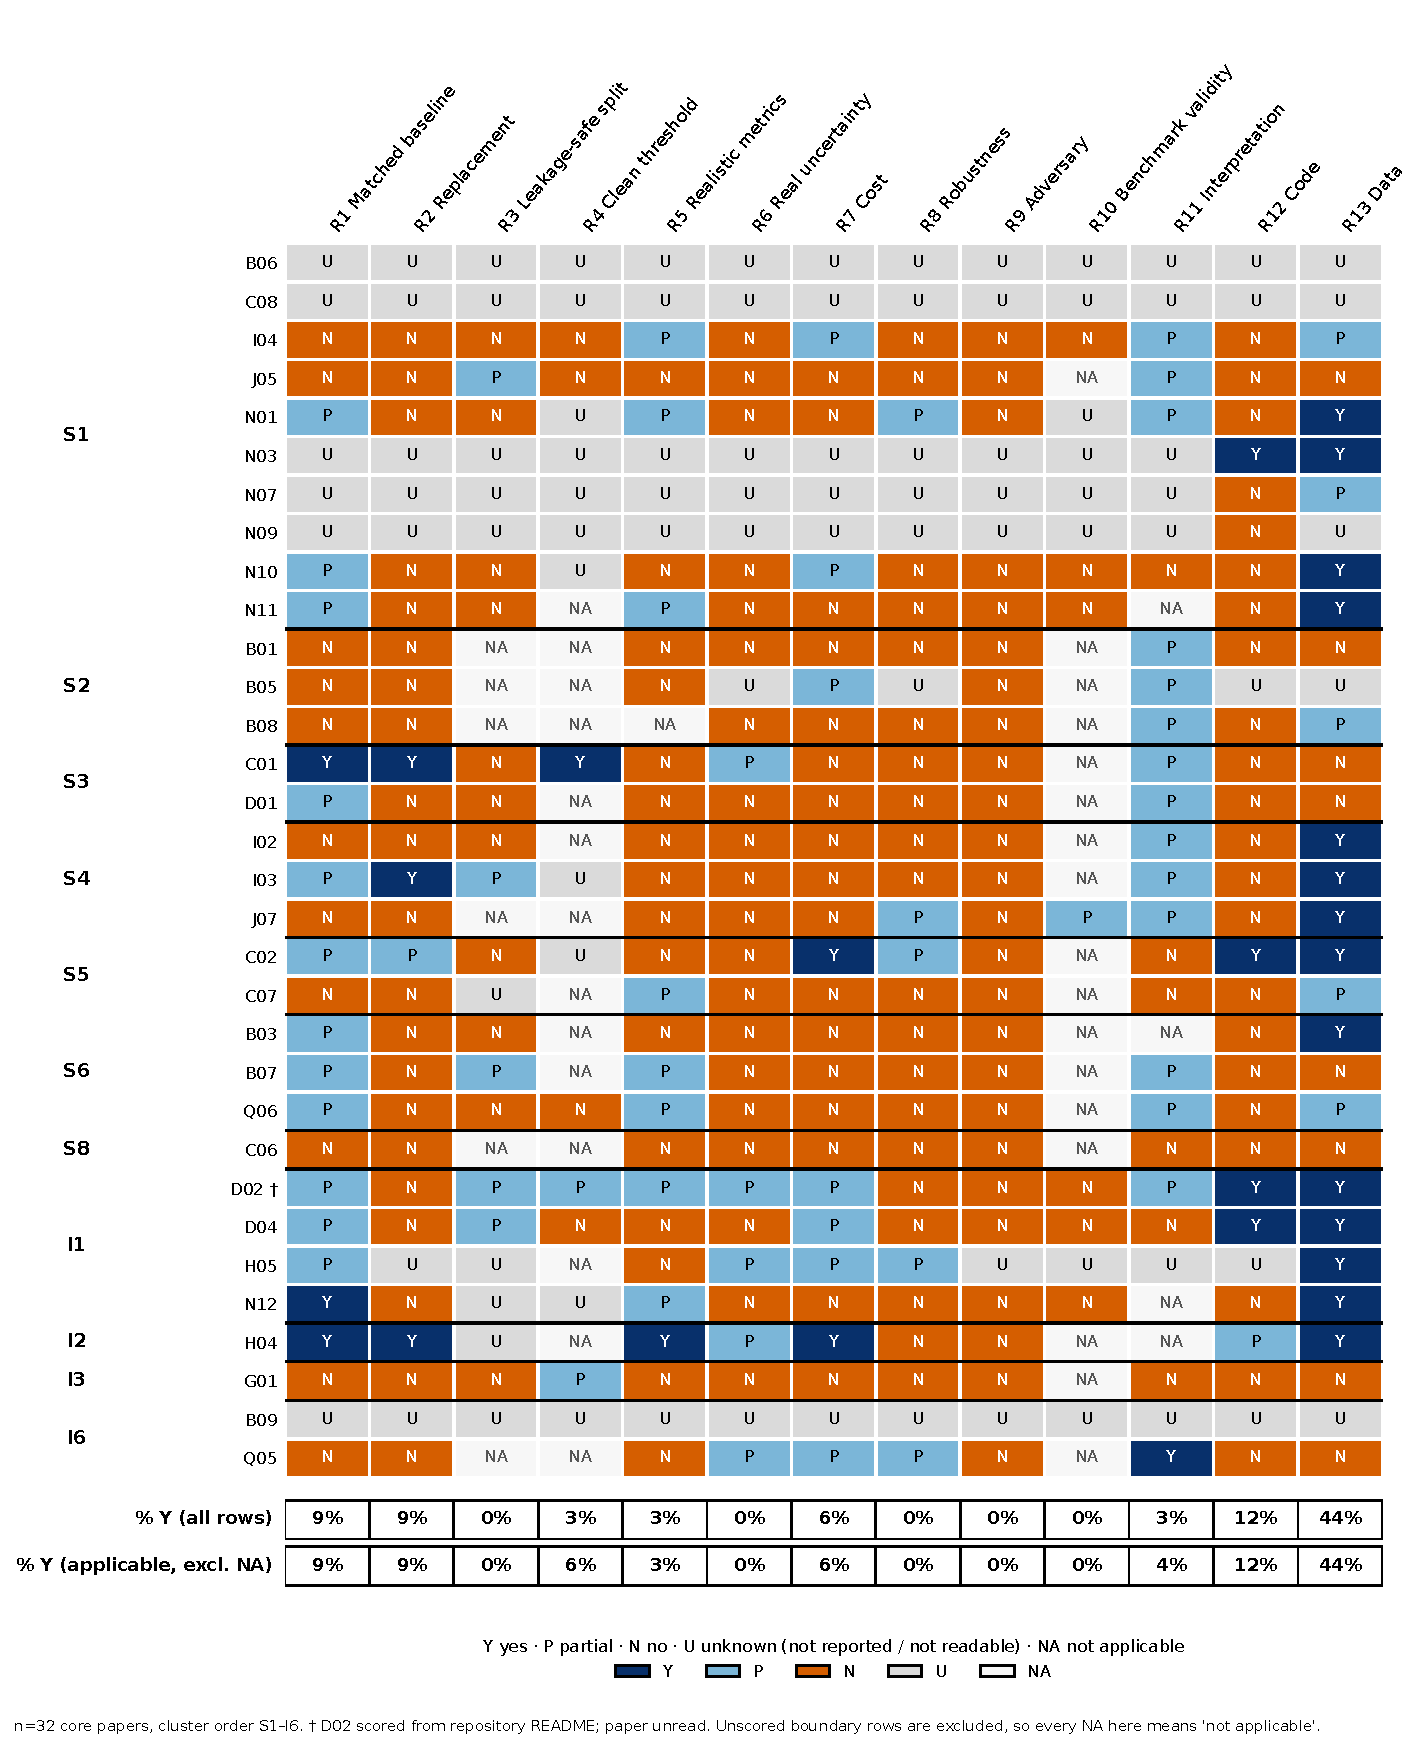
\includegraphics[width=\linewidth,height=0.86\textheight,keepaspectratio]{fig2_rigor_heatmap.pdf}
\caption{Rigour heatmap: R1--R13 for the 32 core papers, grouped by cluster. The bottom rows give the share of papers scoring Y. Every NA means ``not applicable''. D02 (\dag) was scored from its repository README because the paper was not readable.}
\label{fig:rigour}
\end{figure}

\subsection{What the audit can and cannot conclude}
The audit shows that the central claim, that topology adds detection value beyond cheap features, is \emph{almost untested}. It does not show that the claim is false.
\begin{itemize}
  \item The two swap-test losses come from synthetic data (C01) and from a doubtful comparison (C02).
  \item The single win (I03) rests on one host.
  \item Eight papers could be read only as abstracts.
  \item The coding was done by one person with AI assistance, and its reliability is estimated only by the self re-check (Section~\ref{sec:recheck}).
\end{itemize}
The obvious next step is therefore to run the missing test ourselves. That is the purpose of the preregistered experiments in Section~\ref{sec:exp}.

\section{Code-audit findings}
\label{sec:code}

Papers describe their evaluation in a few sentences, but the released code is what produces the numbers. We read six repositories at pinned commits (Table~\ref{tab:code}). Three of them come from the core papers (TAME, TopoGDN and MSF-IDS). The other three are tools we re-test: TADA's implementation \code{tdaad}, PHANTOM, and Fluent Bit's \code{tda} processor.

Every finding below describes what the \emph{released code} does at the stated commit, with file and line numbers so that anyone can check it. None of it is a claim about what the authors ran for their papers.

\begin{table}[ht]
\centering\small
\caption{Summary of the code audit. ``Test information'' means test labels, or statistics computed from the test set, used before scoring.}
\label{tab:code}
\begin{tabularx}{\linewidth}{@{}lllY@{}}
\toprule
Project & Paper & Commit & Main finding \\
\midrule
TAME & D02 & \code{e77c0d9} & Threshold falls back to the test anomaly rate; ``TAME (best)'' is the best detector chosen by test AUROC \\
TopoGDN & D04 & \code{2b8df3b} & Default report is the best F1 over thresholds scored on test labels (inherited from GDN) \\
MSF-IDS & N03 & \code{bb8ccf5} & Random timestamps serve as the persistence filtration on NetFlow data; labels are used while training \\
Fluent Bit \code{tda} & -- & \fillin{\code{25ea7e1}?} & Reported $\beta_k$ counts finite bars only, contrary to its comment; gauges are differenced \\
\code{tdaad} (TADA) & H04 & \code{d103a2c} & README quick-start example fails \\
PHANTOM & -- & \code{8caa25a} & No evaluation problem found (described for E2) \\
\bottomrule
\end{tabularx}
\end{table}

\subsection{TAME (D02)}
TAME~\cite{D02,tame_repo} turns each SMD window into a persistence image, then scores it with shallow detectors. Its repository reports an SMD ROC-AUC of 0.808, against 0.691 for TranAD. At commit \code{e77c0d9}:
\begin{enumerate}
  \item For SMD, PSM and SMAP/MSL, all training labels are set to 0 (\code{utils/data_loaders.py} L52, L176, L224, L268). The validation set is the last 18\% of the training pool, so it contains only normal windows (\code{utils/experiment_core.py} L84--87).
  \item When validation lacks one of the two classes, the threshold falls back to the $1-\textit{expected\_rate}$ quantile of the training scores (\code{experiment_core.py} L105--112). Here \textit{expected\_rate} is the anomaly rate of the \emph{test} labels (L216). The baselines get the same rule (\code{utils/baseline_core.py} L50).
  \item ``TAME (best)'' is the maximum mean \emph{test} AUROC across four detectors and their settings, while each baseline is a single model (\code{consolidate.py} L66--71). The notebooks choose the plotted detector the same way.
  \item The README states that thresholds use ``validation-only threshold selection (never test labels)'' (\code{README.md} L40).
\end{enumerate}
\textbf{What follows.} On these datasets, every threshold-based metric (F1, precision, recall) uses the test anomaly rate, for TAME and the baselines alike. AUROC and AUPRC do not depend on the threshold. But the headline AUROC is a best-of-four pick made on the test set, compared against single baselines. That selection favours TAME. E2 removes both effects: our validation threshold replaces the fallback, and the Isolation Forest variant is fixed in advance.

\subsection{TopoGDN (D04)}
At commit \code{2b8df3b}~\cite{D04}:
\begin{enumerate}
  \item The default reporting mode is \code{-report best} (\code{main.py} L349). In that mode, F1 is computed at 400 thresholds against the \emph{test} labels and the maximum is reported (\code{evaluate.py} L129--143).
  \item Error scores are normalised by the median and inter-quartile range of the test-set errors (\code{evaluate.py} L48--60). These come from test inputs, not labels, so the normalisation is transductive rather than a label leak.
  \item The original GDN code has the same default (d-ailin/GDN at \code{9853899}, \code{main.py} L216).
\end{enumerate}
The paper describes a validation-based threshold (its Sec.~3.6). It does not say which mode produced its main table.

\textbf{What follows.} With the default script, the F1 values are best cases chosen with test labels. The paper's margin over TranAD is under one F1 point on SMD and MSL, so it depends on how TranAD was thresholded. The practice is inherited from GDN and common in this benchmark line, so we report it as a field-level issue, not one specific to TopoGDN.

We did not re-run TopoGDN: its build fails and it requires a GPU. \fillin{one line on the build error, from the logs}

\subsection{MSF-IDS (N03)}
At commit \code{bb8ccf5}~\cite{N03}:
\begin{enumerate}
  \item For the NetFlow (NF) datasets, every record gets a random timestamp in $[0, 86400)$ seconds, and records are then sorted by it (\code{Data/datasets_NF.py} L57--71, L105, L120).
  \item Edge timestamps are the filtration values for persistent homology (\code{Spatial-Frequency Encoders/Spatial Encoder_NAPH.py} L48--52). The diagram becomes a fixed, not learned, persistence image (L52, L65).
  \item The CIC datasets keep their real timestamps (\code{Data/datasets_CIC.py} L56--57, L74--76).
  \item The script builds only a training loader. It evaluates on that same stream, after matching clusters to the true labels (\code{main_Intrusion Detector.py} L76, L353, L384--399). The labels are also used for early stopping (F1 above 0.5) and to accept self-expressive iterations (accuracy above 0.8). \fillin{line numbers}
\end{enumerate}
\textbf{What follows.} On the NF datasets, the filtration orders edges at random, so the persistence features carry no temporal information. Any benefit reported on those datasets cannot come from temporal topology. Evaluating clustering on the stream it was fitted on is common in unsupervised work, but it is not a held-out detection test.

\subsection{Fluent Bit \texttt{tda} processor}
\label{sec:fluentbit}
Fluent Bit, a widely deployed log and metrics agent, ships a \code{tda} processor~\cite{fluentbit_pr11250}, and we found no published evaluation of it. It works as follows:
\begin{enumerate}
  \item it reads metrics only;
  \item it applies a signed $\log(1+|x|)$ transform;
  \item it delay-embeds with $m=3$ and $\tau=1$ over a 60-sample window;
  \item it computes Rips persistence at nine quantile radii and keeps the radius with the largest $\beta_1$;
  \item it emits $\beta_0$, $\beta_1$ and $\beta_2$ as gauges.
\end{enumerate}
We re-implemented it literally as F5. Doing so revealed two behaviours.

\begin{enumerate}
  \item \textbf{What ``$\beta_k$'' counts.} A Betti number at radius $r$ counts the classes \emph{alive} at $r$. The wrapper's comment says it counts the infinite bars, meaning the classes still alive at the chosen radius. The code does the opposite. The Ripser wrapper marks infinite bars with death $=-1$, and the counting loop then drops every bar with death $\le$ birth, so all infinite bars are discarded. Only \emph{finite} bars with persistence of at least $10^{-3}$ are counted, and those are classes that had already died by the chosen radius. So a loop that is still open at the chosen radius is never counted. The reported $\beta_1$ is therefore not the Betti number at that radius, and the radius scan maximises this other quantity. \fillin{wrapper file name and lines, from docs/code\_verification.md \S4}
  \item \textbf{Gauges are differenced.} The rate step in \code{tda.c} (L561--569) runs on every metric type, so gauges such as memory use or CPU percentage are differenced as if they were counters.
\end{enumerate}
\textbf{What follows.} The processor's outputs are well defined, but they do not mean what their names and comments suggest. We keep F5 faithful to the code, including both behaviours. It is reported descriptively and enters no verdict.

\subsection{\texttt{tdaad} (TADA) and PHANTOM}
\begin{itemize}
  \item \textbf{\code{tdaad}}~\cite{tdaad_repo} is the public implementation of TADA~\cite{H04}. At \code{d103a2c}, the quick-start example in its README fails. The example has three sensors, and three points cannot carry an $H_1$ loop in a Rips filtration, because the triangle fills at the same scale as its last edge. \fillin{exact error message and where it is raised} We call the library directly with default parameters in E2.
  \item \textbf{PHANTOM}~\cite{phantom_repo} at \code{8caa25a} (BSD licence) uses Ripser with $H_0$ only. It scores a window by the Wasserstein distance (\code{main.py}; implementation note 42) between a baseline diagram and the diagram of the baseline plus the new window, and it updates the baseline as it goes. This is the scheme described for the PNNL work B06~\citep{B06}. We found no evaluation problem in it. Because it uses $H_0$ only, it measures changes in clustering and spread, not loops.
\end{itemize}

\subsection{Summary}
In three of the six projects, information from the test set enters before scoring:
\begin{itemize}
  \item TAME uses the test anomaly rate and picks its detector by test AUROC;
  \item TopoGDN uses test-optimal thresholds;
  \item MSF-IDS uses labels to stop training.
\end{itemize}
In two more, the topological quantity is not what its description says. MSF-IDS uses a random filtration, and Fluent Bit counts dead bars. None of this shows that the papers' conclusions are wrong. It does show that published numbers cannot be read as fair evidence for topology without re-running the code under clean rules, which is what E1 and E2 do. \fillin{if the authors were contacted, add the date and any reply}

\section{Experiments E1--E5}
\label{sec:exp}

\fillin{Remaining cells are filled in from \code{results/} as runs finish. Every number must come from a result file with its \code{.meta.json} (commit, seeds, versions).}

\subsection{Setup as run}
\begin{itemize}
  \item \textbf{Hardware:} \fillin{CPU, cores, RAM}. Runtimes are per window on one thread and include both feature extraction and scoring.
  \item \textbf{Library versions:} \fillin{from \code{docs/external_versions.md}}.
  \item \textbf{Pinned commits:} TAME \code{e77c0d9}, PHANTOM \code{8caa25a}, \code{tdaad} \code{d103a2c}, Fluent Bit \fillin{commit}.
  \item \textbf{E3 and E2 (our pipelines):} run at commit \code{9c28f8f} with no uncommitted changes, on 28 machines with 5 seeds. Two laptop shutdowns interrupted the run. Each machine's results are saved as soon as it finishes, so the run resumed from the saved machines. One machine whose file was cut off mid-write was deleted and re-run.
  \item \textbf{Test windows:} 3{,}244 positive and 65{,}819 normal across all machines, so positives are 4.7\% of test windows.
  \item \textbf{Data facts checked at access time} (preregistration \S10): \fillin{SMD train/test lengths; SMD sampling interval checked against~\cite{su2019smd} (1 minute assumed, from a secondary source; it affects only false alarms per day); CTU-13 hosts per scenario}.
\end{itemize}

\subsection{E1: TAME as released}
\begin{table}[ht]
\centering\small
\caption{E1: TAME's released code, unchanged, against its reported SMD result.}
\label{tab:e1}
\begin{tabular}{@{}lcc@{}}
\toprule
 & Reported & Our run \\
\midrule
SMD ROC-AUC, ``TAME (best)'' & 0.808 & \pending \\
SMD AUPRC, ``TAME (best)'' & 0.462 & \pending \\
\bottomrule
\end{tabular}
\end{table}

\subsection{E3: swap test on SMD}
Table~\ref{tab:e3} gives the swap test. Adding topological features to the same Isolation Forest raises PR-AUC, and both preregistered comparisons are ``Helps'':
\begin{itemize}
  \item the main gain is $\Delta = +0.054$ [0.035, 0.076];
  \item the swap gain is $\Delta_s = +0.067$ [0.041, 0.097].
\end{itemize}
The gain is consistent across machines: $\Delta > 0$ on 23 of 28 machines, $\Delta < 0$ on 4, and $\Delta = 0$ on 1. Adding topology costs about 1.6\,ms per window.

These are overall results on real SMD anomalies. SMD does not label anomaly types, so they say nothing yet about \emph{which} anomalies topology helps with, and they do not enter P1 or P2. That is E5's job.

The Fluent Bit-style features (F5) score far below every other set. They are reported descriptively and enter no verdict.

\begin{table}[ht]
\centering\footnotesize
\setlength{\tabcolsep}{4pt}
\caption{E3: the same Isolation Forest with different feature sets on SMD. Values are means over 28 machines (5 seeds averaged) with 95\% cluster-bootstrap intervals. Recall is at the 1\% false-alarm threshold. FA/day is false alarms per day, with consecutive alarm windows counted as one event. Runtime is the mean per window, on one thread. Intervals for recall and false alarms are in \code{results/E3}.}
\label{tab:e3}
\begin{tabular}{@{}lccccr@{}}
\toprule
Feature set & PR-AUC & ROC-AUC & Recall & FA/day & ms/win. \\
\midrule
F1 & 0.482 [0.411, 0.559] & 0.858 [0.822, 0.893] & 0.49 & 1.44 & 0.07 \\
F1+F2 & 0.461 [0.390, 0.540] & 0.848 [0.808, 0.887] & 0.45 & 1.79 & 0.59 \\
F1+F3 & 0.529 [0.458, 0.605] & 0.883 [0.851, 0.912] & 0.54 & 1.56 & 1.70 \\
F1+F2+F3 & 0.515 [0.443, 0.594] & 0.876 [0.841, 0.907] & 0.53 & 1.85 & 2.21 \\
F5 (exploratory) & 0.119 [0.093, 0.146] & 0.651 [0.616, 0.685] & 0.10 & 1.66 & 56.0 \\
\midrule
\multicolumn{6}{@{}l}{Preregistered comparisons (PR-AUC)} \\
$\Delta$ = (F1+F2+F3) $-$ (F1+F2) & \multicolumn{5}{l}{+0.054 [0.035, 0.076] \quad \textbf{Helps}} \\
$\Delta_s$ = (F1+F3) $-$ (F1+F2) & \multicolumn{5}{l}{+0.067 [0.041, 0.097] \quad \textbf{Helps}} \\
\midrule
\multicolumn{6}{@{}l}{Exploratory, not preregistered: gain over F1 alone (PR-AUC)} \\
(F1+F2) $-$ F1 & \multicolumn{5}{l}{$-$0.021 [$-$0.035, $-$0.006]} \\
(F1+F3) $-$ F1 & \multicolumn{5}{l}{+0.047 [0.025, 0.072]} \\
(F1+F2+F3) $-$ F1 & \multicolumn{5}{l}{+0.034 [0.012, 0.056]} \\
\bottomrule
\end{tabular}
\end{table}

\paragraph{Exploratory: is the gain just a weak baseline?} The baseline F1+F2 scores \emph{below} F1 alone: adding the simple structure features (F2) slightly hurts this detector. So we also measured each set against F1, as an exploratory check that was not preregistered. Topology still helps there: (F1+F3) $-$ F1 is +0.047 [0.025, 0.072]. The preregistered gain is therefore not an artefact of a weak baseline. Why F2 hurts is open. One candidate is that Isolation Forest picks split features at random, so features that carry no signal dilute it. \fillin{check before claiming}

\paragraph{For scale only.} TAME's repository reports an SMD ROC-AUC of 0.808, and our cheapest set (F1) reaches 0.858. The window length, window labels and threshold rules differ, so these two numbers are \emph{not} comparable. E1 and E2 make the comparison on equal terms.

\subsection{E2: fair re-test on SMD}
\begin{table}[ht]
\centering\footnotesize
\setlength{\tabcolsep}{4pt}
\caption{E2: all methods on the same SMD windows, with the threshold at 1\% false alarms on validation. Our two pipelines are deterministic given the seed, so their rows match E3 exactly. Runtimes are taken from E3, because laptop load differed during the E2 run. Column meanings are as in Table~\ref{tab:e3}.}
\label{tab:e2}
\begin{tabular}{@{}lccccr@{}}
\toprule
Method & PR-AUC & ROC-AUC & Recall & FA/day & ms/win. \\
\midrule
TADA (\code{tdaad}) & \pending & \pending & \pending & \pending & \pending \\
PHANTOM & \pending & \pending & \pending & \pending & \pending \\
TAME (fixed) & \pending & \pending & \pending & \pending & \pending \\
F1+F2 (ours) & 0.461 [0.390, 0.540] & 0.848 [0.808, 0.887] & 0.45 & 1.79 & 0.59 \\
F1+F2+F3 (ours) & 0.515 [0.443, 0.594] & 0.876 [0.841, 0.907] & 0.53 & 1.85 & 2.21 \\
\bottomrule
\end{tabular}
\end{table}

\subsection{E4: CTU-13}
\begin{table}[ht]
\centering\small
\caption{E4: CTU-13, leave-one-scenario-out over 12 scenarios. Supporting evidence only (Section~\ref{sec:limits}).}
\label{tab:e4}
\begin{tabular}{@{}lccc@{}}
\toprule
Comparison & PR-AUC (base) & PR-AUC (with topology) & $\Delta$ [95\% CI] \\
\midrule
F1+F2 vs F1+F2+F3 & \pending & \pending & \pending \\
Z-control vs Z & \pending & \pending & \pending \\
\bottomrule
\end{tabular}
\end{table}
\fillin{per-behaviour-type cells (shape / volume / identity / mixed), with positive and normal window counts}

\subsection{E5: shape versus volume injections}
\begin{table}[ht]
\centering\small
\caption{E5: injected anomalies at the decision magnitude. $\Delta$ = PR-AUC(F1+F2+F3) $-$ PR-AUC(F1+F2).}
\label{tab:e5}
\begin{tabular}{@{}llccl@{}}
\toprule
Type & Injection (decision magnitude) & PR-AUC F1+F2 & $\Delta$ [95\% CI] & Verdict \\
\midrule
S1 & Period $\times 2$ & \pending & \pending & \pending \\
S2 & Phase shift $1/4$ period & \pending & \pending & \pending \\
S3 & Correlation break, fraction 1.0 & \pending & \pending & \pending \\
V1 & Level shift $+2\sigma$ & \pending & \pending & \pending \\
V2 & Spikes $5\sigma$ & \pending & \pending & \pending \\
V3 & Variance $\times 2$ & \pending & \pending & \pending \\
\bottomrule
\end{tabular}
\end{table}
\fillin{Figure: detection versus magnitude, one panel per type; machines skipped for lack of eligible channels}

\subsection{Verdicts}
\begin{itemize}
  \item \textbf{Overall, real SMD anomalies (E3):} topology helps, $\Delta = +0.054$ [0.035, 0.076]. This does not enter P1 or P2.
  \item \textbf{P1} (topology helps on shape): \pending
  \item \textbf{P2} (no added value on volume): \pending
  \item \textbf{P3} (published results shrink): \pending
\end{itemize}

\section{Why: shape versus volume}
\label{sec:why}

\fillin{Write after E5. Planned outline:}
\begin{itemize}
  \item Compare the E5 verdicts with Table~\ref{tab:see}. Did topology add value exactly where the invariance argument said it could, and nowhere else?
  \item For shape types: did F2's cheap structure features already capture the change? If so, topology was able to see the change but added nothing new.
  \item Connect the results back to the literature. The swap-test losses (C01, C02) and the single win (I03): what kind of change did each target (CHG axis)?
  \item State what a practitioner should do: when to try topology, and which cheap baseline to beat first.
\end{itemize}

\section{Limitations and future work}
\label{sec:limits}

\fillin{Draft: extend with anything the experiments reveal.}

\paragraph{Audit.}
\begin{itemize}
  \item One person coded the papers, with AI assistance. Reliability is estimated only by a blind re-score of 7 papers.
  \item Eight core papers could be read only as abstracts.
  \item The search for earlier critical reviews was not completed.
\end{itemize}

\paragraph{Data.}
\begin{itemize}
  \item SMD has no anomaly types, so E2 and E3 give overall results only, and the shape-versus-volume question rests on injections. SMD is also open to the benchmark critiques in~\cite{Q04}. We use it because most TDA papers do, which lets us compare with them directly.
  \item CTU-13 has only 7 distinct normal hosts, 4 of which appear in every scenario. One scenario (10) lacks flow labels. E4 is therefore supporting evidence only.
\end{itemize}

\paragraph{Design.}
\begin{itemize}
  \item E5 is a mechanism test by design. Shape injections keep each channel's mean and variance, and volume injections keep the coupling between channels. It shows what each feature set \emph{can} detect, not how often such anomalies occur in practice.
  \item We use one detector with fixed defaults. Another detector might use topological features differently.
  \item F3 is one reasonable, untuned topology pipeline. A negative result for F3 is not a negative result for every possible topological method.
\end{itemize}

\paragraph{Future work.}
\begin{itemize}
  \item Test against an adversary who knows the features; no paper does (R9).
  \item Replicate I03 on DARPA OpTC with its original hypergraph construction.
  \item Run analyst studies for the exploratory uses (Mapper, motifs), which detection metrics do not capture.
  \item Measure streaming cost at realistic event rates, for Fluent Bit-style deployments.
\end{itemize}


\bibliographystyle{unsrtnat}
\bibliography{references,records}

\appendix
\section{Decision log}
\label{app:decisions}
Ideas that were considered and dropped, and the decisions that shaped the project. Copied from \code{docs/decision_log.md}.

{\small\setlength{\tabcolsep}{4pt}
\begin{longtable}{@{}L{1.9cm}L{4.1cm}L{3.5cm}L{1.6cm}L{3.6cm}@{}}
\toprule
Date & Idea or decision & Evidence checked & Decision & Reason \\
\midrule
\endhead
\fillin{Oct 2026} & TDA for neural-network trojan detection (TopoTrojDetection) & Paper, supplement, code at \code{2e840e1}, model archives & Rejected & Model archives unavailable (HTTP 429); bugs in label loader and preprocessing; close prior work (ArcGen, HTell) \\
\fillin{date} & Path-conditioned PH on microservice traces (RCAEval) & TraceAnomaly, TraceVAE, TraceCRL, ChainLSTM & Not pursued & Path-aware latency modelling already established \\
\fillin{date} & Workload-residual PH on Spark (Exathlon) & TADA, DIVAD & Not pursued & Both ingredients exist; fixed centring leaves correlations unchanged \\
\fillin{date} & PH-based trace sampling & TraceMesh, TraceCRL & Not pursued & Too close to clustering-based sampling \\
\fillin{date} & HPC application-transfer study (Prodigy) & 2025 spectral-topological Deep SVDD paper & Not pursued & Topic already occupied \\
$\le$ 2026-11-12 & Literature audit V1--V3 (76 records; cut-off 14 Oct) & Audit document & Basis for review & A weak evidence base makes the audit itself a contribution \\
2026-11-12 & Critical review of TDA for security and systems telemetry & Davies 2022, Georgiou 2026, 119 logged queries & Adopted & No critical, evaluation-focused review found \\
2026-11-13 & Code-level verification of TAME, TopoGDN, MSF-IDS & Repositories at pinned commits & Adopted & Problems tied to exact lines \\
2026-11-13 to 11-16 & Search rounds 2 and 3; rubric scoring; forward citations & Records CSVs, search logs & Completed & 95 records screened, 32 core papers \\
2026-11-15 & One combined review (security plus systems) & Systems literature alone has about 8 papers & Adopted & Systems alone is too thin \\
2026-11-16 & Review plus a small fair experiment; preregistration v2 & Dataset feasibility checks & Adopted, then revised & A review of weak papers alone would be weak \\
2026-11-17 & Audit plus fair re-evaluation with released code and public data; PHANTOM and zigzag re-test added & Repository and licence checks & Adopted & Evidence must come from our own fair tests \\
2026-11-19 & Preregistration v3: SMD replaces Exathlon; per-host CTU-13 windows; swap test; E5; fixed-default detectors & Flaws found in v2 & Adopted & v2's CTU-13 labelling would break the experiment; SMD validation has no anomalies \\
2026-11-19 & D03 excluded from the core set & No Mapper output on any data & Adopted & Fails inclusion rule 1 in practice \\
\bottomrule
\end{longtable}
}

\section{The 32 core papers}
\label{app:papers}
Group: A swapped, B removed only, C other people's systems, D no comparison, E abstract or code only. ``Claimed'' means the outcome is known only from an abstract or a repository. Generated by \code{report/make_tables.py} from the master CSV.

{\footnotesize\setlength{\tabcolsep}{4pt}
\begin{longtable}{@{}lL{3.8cm}L{2.9cm}llL{1.75cm}L{1.8cm}ll@{}}
\toprule
ID & Title & First author, year & Cl. & Gr. & USE & ISO & OUT & Read \\
\midrule
\endhead
\csname @@input\endcsname tables/core_papers.tex % primitive input: \input is not allowed inside a table
\bottomrule
\end{longtable}
}

\section{Deviations log}
\label{app:deviations}
\fillin{Copy the final \code{deviations_log.md} here after all runs: date, change, reason, affected results.}

\section{Use of AI tools}
\label{app:ai}
\fillin{AI-use note (plan step 21): which tasks used AI assistants (search, extraction, code, drafting), how outputs were checked, and what the author did personally.}


\end{document}
